\documentclass{article}
\usepackage[utf8]{inputenc}
\usepackage{graphicx}
\usepackage{caption}
\usepackage{amsmath}
\usepackage{amssymb}
\usepackage[a4paper, margin=2cm]{geometry}  % <--- Aggiunto per ridurre i bordi

\title{Metodi Matematici}
\author{Nicolò Giuliani}
\date{}

\begin{document}
\maketitle


\section*{0 \, Studiare il dominio}

\textit{Dato che}: \\
\begin{align*}
    f(x) : D \to C
\end{align*}
dove $D$ rappresenta il \textit{dominio} e $C$ il \textit{codominio}.\\

Le regole base del dominio sono:

\begin{align*}
    f(x) = ax + b &\quad \Rightarrow \quad D = \mathbb{R} \\
    f(x) = ax^2 + bx + c &\quad \Rightarrow \quad D = \mathbb{R} \\
    f(x) = \frac{P(x)}{Q(x)} &\quad \Rightarrow \quad D = \mathbb{R} \setminus \{\text{zeri di } Q(x)\} \\
    f(x) = \sqrt{g(x)} &\quad \Rightarrow \quad D = \{x \in \mathbb{R} \mid g(x) \geq 0\} \\
    f(x) = \log(g(x)) &\quad \Rightarrow \quad D = \{x \in \mathbb{R} \mid g(x) > 0\} \\
    f(x) = \ln(x) &\quad \Rightarrow \quad D = \{x \in \mathbb{R} \mid x > 0\} \\
    f(x) = e^x &\quad \Rightarrow \quad D = \mathbb{R} \\
\end{align*}

\textit{Ricorda:} \\
1. il dominio senza un singolo elemento, chiamiamolo $z$, si definisce "$\mathbb{R}\backslash \{z\}$" \\
2. il dominio dato da un insieme \textit{CON} gli estremi si scrive "$[x,y]$" \\
3. il dominio dato da un insieme \textit{SENZA} gli estremi si scrive "$]x, y[$" \\
4. il dominio dato da piu' insiemi si scrive "$[x,y] \cup  [z,k]$", le parentesi possono essere sia quelle che includono o escludono gli estremi.

\pagebreak
\section*{1 \, Studiare la monotonia}

La monotonia si studia attraverso la derivata prima della funzione:
\begin{align*}
    f'(x) = \frac{d}{dx}(f(x))
\end{align*}

Lo studio del segno della derivata prima ci permette di determinare le variazioni della funzione:

\begin{itemize}
    \item $f'(x) > 0$ \quad $\Rightarrow$ \, funzione crescente
    \item $f'(x) < 0$ \quad $\Rightarrow$ \, funzione decrescente
    \item $f'(x) = 0$ \quad $\Rightarrow$ \, possibile punto di massimo, minimo o flesso orizzontale
\end{itemize}

Per individuare i punti di massimo o minimo, si procede nel seguente modo:
\begin{enumerate}
    \item Si risolve l'equazione \( f'(x) = 0 \) per trovare i punti stazionari.
    \item Si calcola la derivsata seconda della funzione:
    \[
        f''(x)<0 \to \text{ massimo}
    \]
    \[
        f''(x)>0 \to \text{ minimo}
    \]
\end{enumerate}
\begin{figure}[h!]
    \centering
    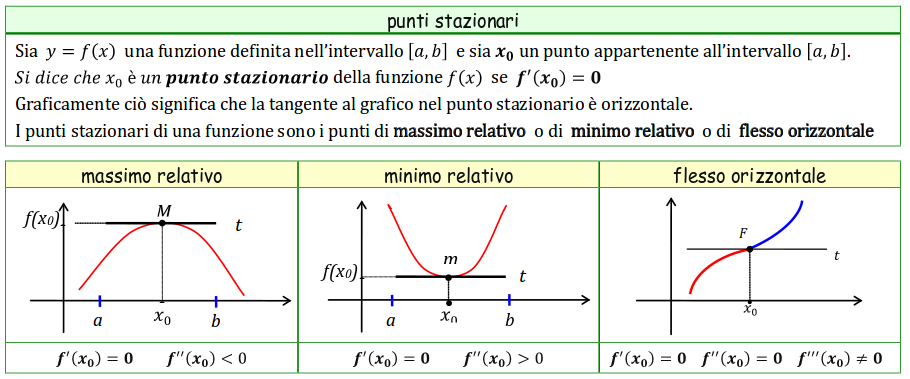
\includegraphics[width=1\textwidth]{max_or_min.png}
    \caption{Massimo o minimo della funzione}
    \label{fig:max_or_min}
\end{figure}

\pagebreak
\section*{2. Studiare il segno}
Studiare il segno di una funzione significa determinare in quali intervalli del dominio la funzione è:
\[
f(x) > 0 \quad \text{(positiva)}
\]
\[
f(x) < 0 \quad \text{(negativa)}
\]
\[
f(x) = 0 \quad \text{(nulla)}
\]

\subsection*{Passi per studiare il segno:}

\paragraph{1. Calcolare il dominio della funzione}
Prima di tutto, è necessario determinare il dominio della funzione, ossia l'insieme dei valori di \(x\) per i quali la funzione è definita. Ad esempio, per una funzione razionale come \(f(x) = \frac{1}{x-2}\), il dominio è \( \mathbb{R} \setminus \{2\} \), poiché la funzione non è definita per \(x = 2\) (dividere per zero).

\paragraph{2. Trovare i valori di \( x \) per cui \( f(x) = 0 \)}
Successivamente, bisogna risolvere l'equazione \( f(x) = 0 \). Gli \( x \) che soddisfano questa equazione sono i \textbf{zeri} della funzione, che dividono la retta reale in intervalli.  
Ecco due esempi di come risolvere:

\subsubsection*{Equazione lineare:}
Se \(f(x) = ax + b\), risolvi l'equazione \( ax + b = 0 \) per ottenere:
\[
x = -\frac{b}{a}
\]

\subsubsection*{Equazione quadratica:}
Se \(f(x) = ax^2 + bx + c\), risolvi l'equazione quadratica \( ax^2 + bx + c = 0 \) usando la formula risolutiva:
\[
x_{1,2} = \frac{-b \pm \sqrt{b^2 - 4ac}}{2a}
\]
Gli zeri della funzione sono i valori di \( x_1 \) e \( x_2 \), se esistono. Se il discriminante (\( b^2 - 4ac \)) è negativo, non ci sono soluzioni reali, e la funzione non ha zeri.

\paragraph{3. Analizzare il segno della funzione negli intervalli}
Una volta trovati gli zeri (e i punti di discontinuità), il dominio si suddivide in intervalli. Ad esempio, se hai trovato \( x = 2 \) come zero, il dominio si suddivide in intervalli come \( (-\infty, 2) \) e \( (2, +\infty) \).

Per ciascun intervallo, scegli un valore \( x \) di test e sostituiscilo nella funzione. In base al segno che ottieni, stabilisci se la funzione è positiva o negativa in quell'intervallo.

\paragraph{Esempi specifici:}

\subsubsection*{Esponenziale:}
La funzione \( f(x) = e^x \) è sempre positiva per ogni \( x \), quindi il segno è:
\[
e^x > 0 \quad \forall x \in \mathbb{R}
\]

\subsubsection*{Logaritmo:}
La funzione \( f(x) = \log(x) \) è definita e positiva per \( x > 1 \), negativa per \( 0 < x < 1 \), e nulla per \( x = 1 \).  
Quindi il segno di \( \log(x) \) è:
\begin{itemize}
    \item Positiva per \( x > 1 \)
    \item Negativa per \( 0 < x < 1 \)
    \item Nulla per \( x = 1 \)
\end{itemize}

\paragraph{4. Costruire una tabella dei segni}
Dopo aver analizzato gli intervalli, costruisci una tabella dei segni, che mostri per ogni intervallo se la funzione è positiva, negativa o nulla.
\begin{figure}[h!]
    \centering
    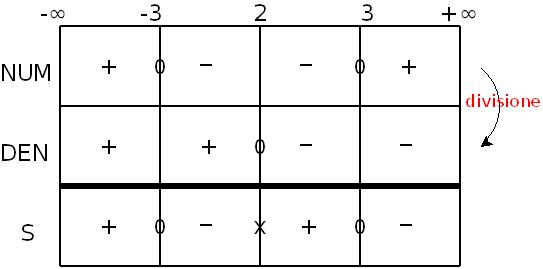
\includegraphics[width=0.7\textwidth]{segni.png}
    \caption{Esempio di tabella dei segni}
    \label{fig:max_or_min}
\end{figure}

\pagebreak
\section*{4. Trovare l’integrale definito tra $[a,b]$}
\begin{align*}
    \int_a^b f(x) \, dx \\
    = [F(x)]_a^b \\
    = F(b) - F(a)
\end{align*}

Le regole base dell'integrazione sono:
\begin{align*}
    \int 1 \, dx = \int dx = x+C \\
    \int kx \, dx = k \int x \, dx
\end{align*}
\begin{align*}
    \int k \, dx &= kx + C \\
    \int x^n \, dx &= \frac{x^{n+1}}{n+1} + C \quad \text{per } n \neq -1 \\
    \int \frac{1}{x} \, dx &= \ln|x| + C \\
    \int e^x \, dx &= e^x + C \\
    \int a^x \, dx &= \frac{a^x}{\ln a} + C \quad \text{per } a\in \mathbb{R} > 0, a \neq 1 \\
\end{align*}
Mentre i metodi comuni per semplificare gli integrali sono:

\begin{enumerate}
    \item \textbf{Integrazione per parti} \\
    Utilizziamo la formula:
    \[
    \int u \, dv = uv - \int v \, du
    \]
    Dove:
    \begin{itemize}
        \item \( u \) è una funzione da derivare
        \item \( dv \) è una funzione da integrare
    \end{itemize}

    \item \textbf{Integrazione per sostituzione} \textit{(Non cosigliata per metodi)}\\
    Serve quando l'integrale contiene una funzione composta. Si pone:
    \[
    u = g(x) \quad \Rightarrow \quad du = g'(x)\, dx
    \]
    Allora l'integrale diventa:
    \[
    \int f(g(x)) \cdot g'(x) \, dx = \int f(u) \, du
    \]
\end{enumerate}
\textit{Nota bene:} nel caso di integrali definiti, una volta effettuata la sostituzione \( u = g(x) \), è necessario ricalcolare gli estremi di integrazione in termini della nuova variabile. Se l'integrale iniziale è:
\[
\int_a^b f(g(x)) \cdot g'(x) \, dx
\]
dopo la sostituzione diventa:
\[
\int_{u(a)}^{u(b)} f(u) \, du
\]
dove \( u(a) = g(a) \) e \( u(b) = g(b) \). \\
\textbf{Alcune formule comuni di integrazione}

\begin{align*}
    \int f(x)dx = \frac{1}{1} \int f(x)dx = \frac{z}{z} \int f(x)dx \quad (\text{con }z\in \mathbb{R}\backslash \{z\}) \\
\end{align*}
\begin{align*}
    \int \frac{f'(x)}{f(x)} \, dx &= \ln|f(x)| + C \\
    \int \frac{f'(x)}{(f(x))^2} \, dx &= -\frac{1}{f(x)} + C \\
    \int \frac{1}{\sqrt{x^2 + a^2}} \, dx &= \ln \left| x + \sqrt{x^2 + a^2} \right| + C \\
    \int \frac{1}{\sqrt{x^2 - a^2}} \, dx &= \ln \left| x + \sqrt{x^2 - a^2} \right| + C \\
\end{align*}

\pagebreak
\section*{6. Determinare l’equazione della retta tangente alla funzione data per il punto di ascissa $x_0$}
La forumula per l'equazione della retta tangente in un punto e':
\begin{align*}
    t(x)=f'(x_0)f(x-x_0)+f(x_0)
\end{align*}
1. calcoliamo $f'(x)$, poi inseriamo $x_0$ e otteniamo $f(x_0)$. \\
2. calcoliamo il valore di $f(x_0)$. \\
3. moltiplichiamo e sommiamo per ottenere la funzione $t(x)$.

\vspace{2em}
\section*{7. Determinare il valore del parametro $c$, tale che la funzione sia continua}
Dato:
\begin{align*}
    f(x) = \begin{cases}
        g(x) \quad &\text{se } x < p \\
        h(x) \quad &\text{se } x \geq p \\
    \end{cases}
\end{align*}

Una funzione è continua in un punto \( x = p \) se:
\begin{align*}
    \lim_{x \to p^-} f(x) = \lim_{x \to p^+} f(x) = f(p)
\end{align*}

\textbf{Per esempio:}
\begin{align*}
    f(x) = \begin{cases}
        x^2 + 1 \quad &\text{se } x < 2 \\
        cx + 1 \quad &\text{se } x \geq 2 \\
    \end{cases}
\end{align*}

Calcoliamo il limite sinistro:
\begin{align*}
    \lim_{x \to 2^-} f(x) = \lim_{x \to 2^-} (x^2 + 1) = 2^2 + 1 = 5
\end{align*}

Calcoliamo il limite destro:
\begin{align*}
    \lim_{x \to 2^+} f(x) = \lim_{x \to 2^+} (cx + 1) = 2c + 1
\end{align*}

Imponiamo la continuità:
\begin{align*}
    2c + 1 = 5 \Rightarrow c = 2
\end{align*}

\textbf{Conclusione:} per rendere \( f(x) \) continua in \( x = 2 \), il parametro deve essere \( c = 2 \).

\subsection*{Calcolo del codominio}
Dato che \( D = [a, b] \), se la funzione è continua e monotona, il codominio sarà:
\begin{align*}
    C = [f(a), f(b)] 
\end{align*}

\subsection*{Iniettiva}
Una funzione è \textbf{iniettiva} se ogni elemento del dominio ha un'immagine diversa:
\[
f(a) \neq f(b) \quad \forall a, b \in D, \; a \neq b
\]

\subsection*{Suriettiva}
Una funzione è \textbf{suriettiva} se ogni elemento del codominio è immagine di almeno un elemento del dominio:
\[
\forall y \in C, \; \exists x \in D \text{ tale che } f(x) = y
\]

\subsection*{Biettiva}
Una funzione è \textbf{biettiva} se è sia iniettiva che suriettiva: ogni elemento del codominio è raggiunto da uno e un solo elemento del dominio.
\begin{figure}[h!]
    \centering
    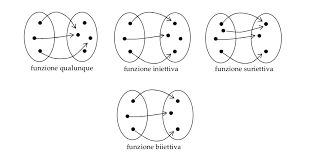
\includegraphics[width=0.7\textwidth]{iniettiva_suriettiva.png}
    \caption{Visione grafica del carattere delle funzioni, \textit{a sinistra abbiamo il dominio e a destra il codominio}}
    \label{fig:max_or_min}
\end{figure}






\end{document}